%% bare_conf.tex
%% V1.3
%% 2007/01/11
%% by Michael Shell
%% See:
%% http://www.michaelshell.org/
%% for current contact information.
%%
%% This is a skeleton file demonstrating the use of IEEEtran.cls
%% (requires IEEEtran.cls version 1.7 or later) with an IEEE conference paper.
%%
%% Support sites:
%% http://www.michaelshell.org/tex/ieeetran/
%% http://www.ctan.org/tex-archive/macros/latex/contrib/IEEEtran/
%% and
%% http://www.ieee.org/

%%*************************************************************************
%% Legal Notice:
%% This code is offered as-is without any warranty either expressed or
%% implied; without even the implied warranty of MERCHANTABILITY or
%% FITNESS FOR A PARTICULAR PURPOSE! 
%% User assumes all risk.
%% In no event shall IEEE or any contributor to this code be liable for
%% any damages or losses, including, but not limited to, incidental,
%% consequential, or any other damages, resulting from the use or misuse
%% of any information contained here.
%%
%% All comments are the opinions of their respective authors and are not
%% necessarily endorsed by the IEEE.
%%
%% This work is distributed under the LaTeX Project Public License (LPPL)
%% ( http://www.latex-project.org/ ) version 1.3, and may be freely used,
%% distributed and modified. A copy of the LPPL, version 1.3, is included
%% in the base LaTeX documentation of all distributions of LaTeX released
%% 2003/12/01 or later.
%% Retain all contribution notices and credits.
%% ** Modified files should be clearly indicated as such, including  **
%% ** renaming them and changing author support contact information. **
%%
%% File list of work: IEEEtran.cls, IEEEtran_HOWTO.pdf, bare_adv.tex,
%%                    bare_conf.tex, bare_jrnl.tex, bare_jrnl_compsoc.tex
%%*************************************************************************

% *** Authors should verify (and, if needed, correct) their LaTeX system  ***
% *** with the testflow diagnostic prior to trusting their LaTeX platform ***
% *** with production work. IEEE's font choices can trigger bugs that do  ***
% *** not appear when using other class files.                            ***
% The testflow support page is at:
% http://www.michaelshell.org/tex/testflow/



% Note that the a4paper option is mainly intended so that authors in
% countries using A4 can easily print to A4 and see how their papers will
% look in print - the typesetting of the document will not typically be
% affected with changes in paper size (but the bottom and side margins will).
% Use the testflow package mentioned above to verify correct handling of
% both paper sizes by the user's LaTeX system.
%
% Also note that the "draftcls" or "draftclsnofoot", not "draft", option
% should be used if it is desired that the figures are to be displayed in
% draft mode.
%
\documentclass[10pt, conference, compsocconf]{IEEEtran}
% Add the compsocconf option for Computer Society conferences.
%
% If IEEEtran.cls has not been installed into the LaTeX system files,
% manually specify the path to it like:
% \documentclass[conference]{../sty/IEEEtran}





% Some very useful LaTeX packages include:
% (uncomment the ones you want to load)


% *** MISC UTILITY PACKAGES ***
%
%\usepackage{ifpdf}
% Heiko Oberdiek's ifpdf.sty is very useful if you need conditional
% compilation based on whether the output is pdf or dvi.
% usage:
% \ifpdf
%   % pdf code
% \else
%   % dvi code
% \fi
% The latest version of ifpdf.sty can be obtained from:
% http://www.ctan.org/tex-archive/macros/latex/contrib/oberdiek/
% Also, note that IEEEtran.cls V1.7 and later provides a builtin
% \ifCLASSINFOpdf conditional that works the same way.
% When switching from latex to pdflatex and vice-versa, the compiler may
% have to be run twice to clear warning/error messages.






% *** CITATION PACKAGES ***
%
\usepackage{cite}
% cite.sty was written by Donald Arseneau
% V1.6 and later of IEEEtran pre-defines the format of the cite.sty package
% \cite{} output to follow that of IEEE. Loading the cite package will
% result in citation numbers being automatically sorted and properly
% "compressed/ranged". e.g., [1], [9], [2], [7], [5], [6] without using
% cite.sty will become [1], [2], [5]--[7], [9] using cite.sty. cite.sty's
% \cite will automatically add leading space, if needed. Use cite.sty's
% noadjust option (cite.sty V3.8 and later) if you want to turn this off.
% cite.sty is already installed on most LaTeX systems. Be sure and use
% version 4.0 (2003-05-27) and later if using hyperref.sty. cite.sty does
% not currently provide for hyperlinked citations.
% The latest version can be obtained at:
% http://www.ctan.org/tex-archive/macros/latex/contrib/cite/
% The documentation is contained in the cite.sty file itself.






% *** GRAPHICS RELATED PACKAGES ***
%
\ifCLASSINFOpdf
  \usepackage[pdftex]{graphicx}
  % declare the path(s) where your graphic files are
  % \graphicspath{{../pdf/}{../jpeg/}}
  % and their extensions so you won't have to specify these with
  % every instance of \includegraphics
  % \DeclareGraphicsExtensions{.pdf,.jpeg,.png}
\else
  % or other class option (dvipsone, dvipdf, if not using dvips). graphicx
  % will default to the driver specified in the system graphics.cfg if no
  % driver is specified.
  % \usepackage[dvips]{graphicx}
  % declare the path(s) where your graphic files are
  % \graphicspath{{../eps/}}
  % and their extensions so you won't have to specify these with
  % every instance of \includegraphics
  % \DeclareGraphicsExtensions{.eps}
\fi
% graphicx was written by David Carlisle and Sebastian Rahtz. It is
% required if you want graphics, photos, etc. graphicx.sty is already
% installed on most LaTeX systems. The latest version and documentation can
% be obtained at: 
% http://www.ctan.org/tex-archive/macros/latex/required/graphics/
% Another good source of documentation is "Using Imported Graphics in
% LaTeX2e" by Keith Reckdahl which can be found as epslatex.ps or
% epslatex.pdf at: http://www.ctan.org/tex-archive/info/
%
% latex, and pdflatex in dvi mode, support graphics in encapsulated
% postscript (.eps) format. pdflatex in pdf mode supports graphics
% in .pdf, .jpeg, .png and .mps (metapost) formats. Users should ensure
% that all non-photo figures use a vector format (.eps, .pdf, .mps) and
% not a bitmapped formats (.jpeg, .png). IEEE frowns on bitmapped formats
% which can result in "jaggedy"/blurry rendering of lines and letters as
% well as large increases in file sizes.
%
% You can find documentation about the pdfTeX application at:
% http://www.tug.org/applications/pdftex





% *** MATH PACKAGES ***
%
%\usepackage[cmex10]{amsmath}
% A popular package from the American Mathematical Society that provides
% many useful and powerful commands for dealing with mathematics. If using
% it, be sure to load this package with the cmex10 option to ensure that
% only type 1 fonts will utilized at all point sizes. Without this option,
% it is possible that some math symbols, particularly those within
% footnotes, will be rendered in bitmap form which will result in a
% document that can not be IEEE Xplore compliant!
%
% Also, note that the amsmath package sets \interdisplaylinepenalty to 10000
% thus preventing page breaks from occurring within multiline equations. Use:
%\interdisplaylinepenalty=2500
% after loading amsmath to restore such page breaks as IEEEtran.cls normally
% does. amsmath.sty is already installed on most LaTeX systems. The latest
% version and documentation can be obtained at:
% http://www.ctan.org/tex-archive/macros/latex/required/amslatex/math/





% *** SPECIALIZED LIST PACKAGES ***
%
%\usepackage{algorithmic}
% algorithmic.sty was written by Peter Williams and Rogerio Brito.
% This package provides an algorithmic environment fo describing algorithms.
% You can use the algorithmic environment in-text or within a figure
% environment to provide for a floating algorithm. Do NOT use the algorithm
% floating environment provided by algorithm.sty (by the same authors) or
% algorithm2e.sty (by Christophe Fiorio) as IEEE does not use dedicated
% algorithm float types and packages that provide these will not provide
% correct IEEE style captions. The latest version and documentation of
% algorithmic.sty can be obtained at:
% http://www.ctan.org/tex-archive/macros/latex/contrib/algorithms/
% There is also a support site at:
% http://algorithms.berlios.de/index.html
% Also of interest may be the (relatively newer and more customizable)
% algorithmicx.sty package by Szasz Janos:
% http://www.ctan.org/tex-archive/macros/latex/contrib/algorithmicx/




% *** ALIGNMENT PACKAGES ***
%
%\usepackage{array}
% Frank Mittelbach's and David Carlisle's array.sty patches and improves
% the standard LaTeX2e array and tabular environments to provide better
% appearance and additional user controls. As the default LaTeX2e table
% generation code is lacking to the point of almost being broken with
% respect to the quality of the end results, all users are strongly
% advised to use an enhanced (at the very least that provided by array.sty)
% set of table tools. array.sty is already installed on most systems. The
% latest version and documentation can be obtained at:
% http://www.ctan.org/tex-archive/macros/latex/required/tools/


%\usepackage{mdwmath}
%\usepackage{mdwtab}
% Also highly recommended is Mark Wooding's extremely powerful MDW tools,
% especially mdwmath.sty and mdwtab.sty which are used to format equations
% and tables, respectively. The MDWtools set is already installed on most
% LaTeX systems. The lastest version and documentation is available at:
% http://www.ctan.org/tex-archive/macros/latex/contrib/mdwtools/


% IEEEtran contains the IEEEeqnarray family of commands that can be used to
% generate multiline equations as well as matrices, tables, etc., of high
% quality.


%\usepackage{eqparbox}
% Also of notable interest is Scott Pakin's eqparbox package for creating
% (automatically sized) equal width boxes - aka "natural width parboxes".
% Available at:
% http://www.ctan.org/tex-archive/macros/latex/contrib/eqparbox/





% *** SUBFIGURE PACKAGES ***
%\usepackage[tight,footnotesize]{subfigure}
% subfigure.sty was written by Steven Douglas Cochran. This package makes it
% easy to put subfigures in your figures. e.g., "Figure 1a and 1b". For IEEE
% work, it is a good idea to load it with the tight package option to reduce
% the amount of white space around the subfigures. subfigure.sty is already
% installed on most LaTeX systems. The latest version and documentation can
% be obtained at:
% http://www.ctan.org/tex-archive/obsolete/macros/latex/contrib/subfigure/
% subfigure.sty has been superceeded by subfig.sty.



%\usepackage[caption=false]{caption}
%\usepackage[font=footnotesize]{subfig}
% subfig.sty, also written by Steven Douglas Cochran, is the modern
% replacement for subfigure.sty. However, subfig.sty requires and
% automatically loads Axel Sommerfeldt's caption.sty which will override
% IEEEtran.cls handling of captions and this will result in nonIEEE style
% figure/table captions. To prevent this problem, be sure and preload
% caption.sty with its "caption=false" package option. This is will preserve
% IEEEtran.cls handing of captions. Version 1.3 (2005/06/28) and later 
% (recommended due to many improvements over 1.2) of subfig.sty supports
% the caption=false option directly:
%\usepackage[caption=false,font=footnotesize]{subfig}
%
% The latest version and documentation can be obtained at:
% http://www.ctan.org/tex-archive/macros/latex/contrib/subfig/
% The latest version and documentation of caption.sty can be obtained at:
% http://www.ctan.org/tex-archive/macros/latex/contrib/caption/




% *** FLOAT PACKAGES ***
%
%\usepackage{fixltx2e}
% fixltx2e, the successor to the earlier fix2col.sty, was written by
% Frank Mittelbach and David Carlisle. This package corrects a few problems
% in the LaTeX2e kernel, the most notable of which is that in current
% LaTeX2e releases, the ordering of single and double column floats is not
% guaranteed to be preserved. Thus, an unpatched LaTeX2e can allow a
% single column figure to be placed prior to an earlier double column
% figure. The latest version and documentation can be found at:
% http://www.ctan.org/tex-archive/macros/latex/base/



%\usepackage{stfloats}
% stfloats.sty was written by Sigitas Tolusis. This package gives LaTeX2e
% the ability to do double column floats at the bottom of the page as well
% as the top. (e.g., "\begin{figure*}[!b]" is not normally possible in
% LaTeX2e). It also provides a command:
%\fnbelowfloat
% to enable the placement of footnotes below bottom floats (the standard
% LaTeX2e kernel puts them above bottom floats). This is an invasive package
% which rewrites many portions of the LaTeX2e float routines. It may not work
% with other packages that modify the LaTeX2e float routines. The latest
% version and documentation can be obtained at:
% http://www.ctan.org/tex-archive/macros/latex/contrib/sttools/
% Documentation is contained in the stfloats.sty comments as well as in the
% presfull.pdf file. Do not use the stfloats baselinefloat ability as IEEE
% does not allow \baselineskip to stretch. Authors submitting work to the
% IEEE should note that IEEE rarely uses double column equations and
% that authors should try to avoid such use. Do not be tempted to use the
% cuted.sty or midfloat.sty packages (also by Sigitas Tolusis) as IEEE does
% not format its papers in such ways.





% *** PDF, URL AND HYPERLINK PACKAGES ***
%
%\usepackage{url}
% url.sty was written by Donald Arseneau. It provides better support for
% handling and breaking URLs. url.sty is already installed on most LaTeX
% systems. The latest version can be obtained at:
% http://www.ctan.org/tex-archive/macros/latex/contrib/misc/
% Read the url.sty source comments for usage information. Basically,
% \url{my_url_here}.





% *** Do not adjust lengths that control margins, column widths, etc. ***
% *** Do not use packages that alter fonts (such as pslatex).         ***
% There should be no need to do such things with IEEEtran.cls V1.6 and later.
% (Unless specifically asked to do so by the journal or conference you plan
% to submit to, of course. )


% correct bad hyphenation here
\hyphenation{op-tical net-works semi-conduc-tor}


\begin{document}
%
% paper title
% can use linebreaks \\ within to get better formatting as desired
\title{SLA-Guided Data Integration on Cloud Environments}


% author names and affiliations
% use a multiple column layout for up to two different
% affiliations

\author{
\IEEEauthorblockN{Nadia Bennani}
\IEEEauthorblockA{LIRIS, INSA-LYON \\
Lyon, France\\
nadia.bennani@insa-lyon.fr}
\and
\IEEEauthorblockN{Chirine Ghedira-Guegan}
\IEEEauthorblockA{IAE Universit\'e de Lyon 3\\
Lyon, France\\
chirine.ghedira-guegan@univ-lyon3.fr}
\and
\IEEEauthorblockN{Martin A. Musicante}
\IEEEauthorblockA{DIMAp, UFRN\\
Natal, Brazil\\
mam@dimap.ufrn.br}
\and
\IEEEauthorblockN{Genoveva Vargas-Solar}
\IEEEauthorblockA{CNRS, LIG-LAFMIA\\
St. Martin D'H\`eres, France\\
genoveva.vargas@imag.fr}
}

% conference papers do not typically use \thanks and this command
% is locked out in conference mode. If really needed, such as for
% the acknowledgment of grants, issue a \IEEEoverridecommandlockouts
% after \documentclass

% for over three affiliations, or if they all won't fit within the width
% of the page, use this alternative format:
% 
%\author{\IEEEauthorblockN{Michael Shell\IEEEauthorrefmark{1},
%Homer Simpson\IEEEauthorrefmark{2},
%James Kirk\IEEEauthorrefmark{3}, 
%Montgomery Scott\IEEEauthorrefmark{3} and
%Eldon Tyrell\IEEEauthorrefmark{4}}
%\IEEEauthorblockA{\IEEEauthorrefmark{1}School of Electrical and Computer Engineering\\
%Georgia Institute of Technology,
%Atlanta, Georgia 30332--0250\\ Email: see http://www.michaelshell.org/contact.html}
%\IEEEauthorblockA{\IEEEauthorrefmark{2}Twentieth Century Fox, Springfield, USA\\
%Email: homer@thesimpsons.com}
%\IEEEauthorblockA{\IEEEauthorrefmark{3}Starfleet Academy, San Francisco, California 96678-2391\\
%Telephone: (800) 555--1212, Fax: (888) 555--1212}
%\IEEEauthorblockA{\IEEEauthorrefmark{4}Tyrell Inc., 123 Replicant Street, Los Angeles, California 90210--4321}}




% use for special paper notices
%\IEEEspecialpapernotice{(Invited Paper)}




% make the title area
\maketitle


\begin{abstract}
Cloud computing is becoming a popular model for storing and accessing data on the Internet.
The model includes financial cost for using the services provided on the Cloud, as well as other constraints like QoS and non-functional requirements.
Service Level Agreements implement the contracts between the cloud provider and the users. 
In this paper, we propose a data integration architecture for querying multiple clouds.
Our approach uses SLA to guide the discovery and integration process.
\end{abstract}

\begin{IEEEkeywords}
SLA; Cloud Computing; Data Integration;
\end{IEEEkeywords}


% For peer review papers, you can put extra information on the cover
% page as needed:
% \ifCLASSOPTIONpeerreview
% \begin{center} \bfseries EDICS Category: 3-BBND \end{center}
% \fi
%
% For peerreview papers, this IEEEtran command inserts a page break and
% creates the second title. It will be ignored for other modes.
\IEEEpeerreviewmaketitle



\section{Introduction}
% no \IEEEPARstart
%This demo file is intended to serve as a ``starter file''
%for IEEE conference papers produced under \LaTeX\ using
%IEEEtran.cls version 1.7 and later.
%
%All manuscripts must be in English. These guidelines include complete descriptions of the fonts, spacing, and related information for producing your proceedings manuscripts. Please follow them and if you have any questions, direct them to the production editor in charge of your proceedings at Conference Publishing Services (CPS): Phone +1 (714) 821-8380 or Fax +1 (714) 761-1784.
% You must have at least 2 lines in the paragraph with the drop letter
% (should never be an issue)

The recent emergence of  the cloud paradigm opens new challenges to data processing. Indeed, unlimited access to cloud resources and the "pay as U go" model change the hypothesis for processing big data collections.
Nevertheless, integrating and processing heterogeneous data collections, calls for efficient methods for correlating, associating, filtering those data taking into consideration their “structural” characteristics (due to the different data models) but also their quality, e.g., trust, freshness, provenance, partial or total consistency.

Existing data integration techniques have to be revisited in order to integrate data that are both weakly curated and described through metadata or schemas. 
This issue is highlighted by the numerous resources deployed by several providers  on the cloud, and for which Service Level Agreement Contracts (SLA) are associated. 
In the current model, users sign a contract with one or many cloud providers.
The contract is materialized as an \textit{user SLA}. 
Each user has his own constraints and quality of service requirements when querying data on the cloud. 

Let us illustrate our our problem by an example in the domain of energy management.
We are interested in queries like: \textit{What is the list of energy providers that can provision 1000 KW-h, in the next 10 seconds, that are close to my city, with a cost of 0,50 Euro/KW-h and that are labelled as green?}. 
We consider a simplified SLA cloud contract inspired in the lowest contract provided by Azure: \textit{cost of \$0,05 cents per call,  8~GB of I/O volume/month, free data transfer cost within the same region,  01~GB of storage.} 
The user is ready to pay a maximum of \textit{\$5 as total query cost}; she requests that only  \textit{green} energy providers are listed (provenance), with at least  \textit{85$\%$} of precision of provided data, even if they are not fresh; she requires an availability rate of at least 90$\%$ and a response time of  \textit{0,01 s}. 

% which differs from the users’ SLA.
    The question is how can the user  obtain efficiently results for her queries that meet her Q\&S requirements while respecting her subscribed contracts with the cloud and also without neglecting services contracts, especially for queries to several services deployed eventually on different clouds?
%    needs especially for those that requires requests especially complex ones that need data service compositions,  can met Quality Of Service requirements expressed by their consumers and Service Level Agreement Contracts (SLA), both at the cloud level and at the service level. 
%présenter le type de requête et le contexte d'utilisation du type de reque^te 

To our knowledge, projects and deployments of SLAs in the context of Cloud Computing aim and rely on two principles: (i) The negotiation of conditions, which are statically agreed between the parts (\cite{5547150,Dastjerdi:2012:DOA:2275356.2275360,Ortiz:2013:VPS:2486767.2486772} (ii) The monitoring of these conditions during the use of cloud resources in order to detect SLA contract violation (\cite{6274042,5614035}).


Our work intends to address data integration on a  cloud guided by the SLA exported by different cloud providers and by QoS measures associated to data collections properties: trust, privacy, economic cost. 
This implies several granularities of SLA: first, at the cloud level; the SLA ensured by providers regarding data; then at the service level, as unit for accessing and processing data, to be sure to fit particular service needs; and finally at the integration level i.e the possibility to process, correlate and integrate big data collections distributed along different cloud storage supports, providing different quality properties to data (trust, privacy, reliability, etc).
The goal is to propose an SLA guided data integration system exported as a distributed DaaS by a set of clouds providers that handles the SLA interoperability and collaboration. 

%comment on pense faire pour répondre à la problématique en se basant sur le use case

In this paper, we present our approach and optimized economic driven and client-oriented data integration (lookup, aggregation, correlation) strategies adapted to the vision of the economic model of the cloud.
We aim at (i) accepting partial results delivered on demand or under predefined subscription models that can affect the quality of the results; (ii) accepting specific data duplication that can respect privacy but ensure data availability; (iii) accepting to launch a task that contributes to an integration on a first cloud whose SLA verifies security requirement rather than a more powerful cloud but with less security guarantees in the SLA. 
%The paper is outlined as follows: Section 2 describes the service architecture. Section 3 presents our Integration SLA structure that allows to optimize further query execution by minimizing time negociation and time execution when similar partial or total queries has been already executed. 

\section{The SLA-guided  data integration approach}
Our SLA guided data  integration approach proposes three steps starting from the processing of the request to the delivery of the result sets.
Given an expressed query and a set of Q\&S preferences: cost, data provenance, service reputation, execution deadline and so on, the system processes in three steps, as follows: first (i) an SLA derivation computation is performed to filter possible data and services providers.
This may be done using a set of matching algorithms based on  graph structures and RDF specification.
Then, (ii) a query rewriting is done, in term of possible service compositions giving partial or exhaustive  results according to SLAs content; and finally, (iii) the results are integrated into an answer. 
These steps generate intermediate results that are stored as knowledge in order to reduce the overhead of the query evaluation process. 
The whole process is monitored to determine whether a computed SLA is being honoured while a query is evaluated. 

%We can now describe our SLA-guided data integration As a service (SLAG-DIAAS) architecture.
%
%\section{The SLA-GIDAAS architecture}
Figure~\ref{fig_sim} shows the SLAG-DIAAS architecture of an SLA guided data integration system that is supported by data services which are data providers deployed in a cloud and that provide agreed SLAs. 
The architecture keeps a \textit{directory} together with meta-data about the way queries are evaluated for producing results.
The system uses this information by query processing and monitoring modules for rewriting queries according to given quality of service (QoS) preferences expressed by a data consumer.
\begin{figure}[!t]
\centering
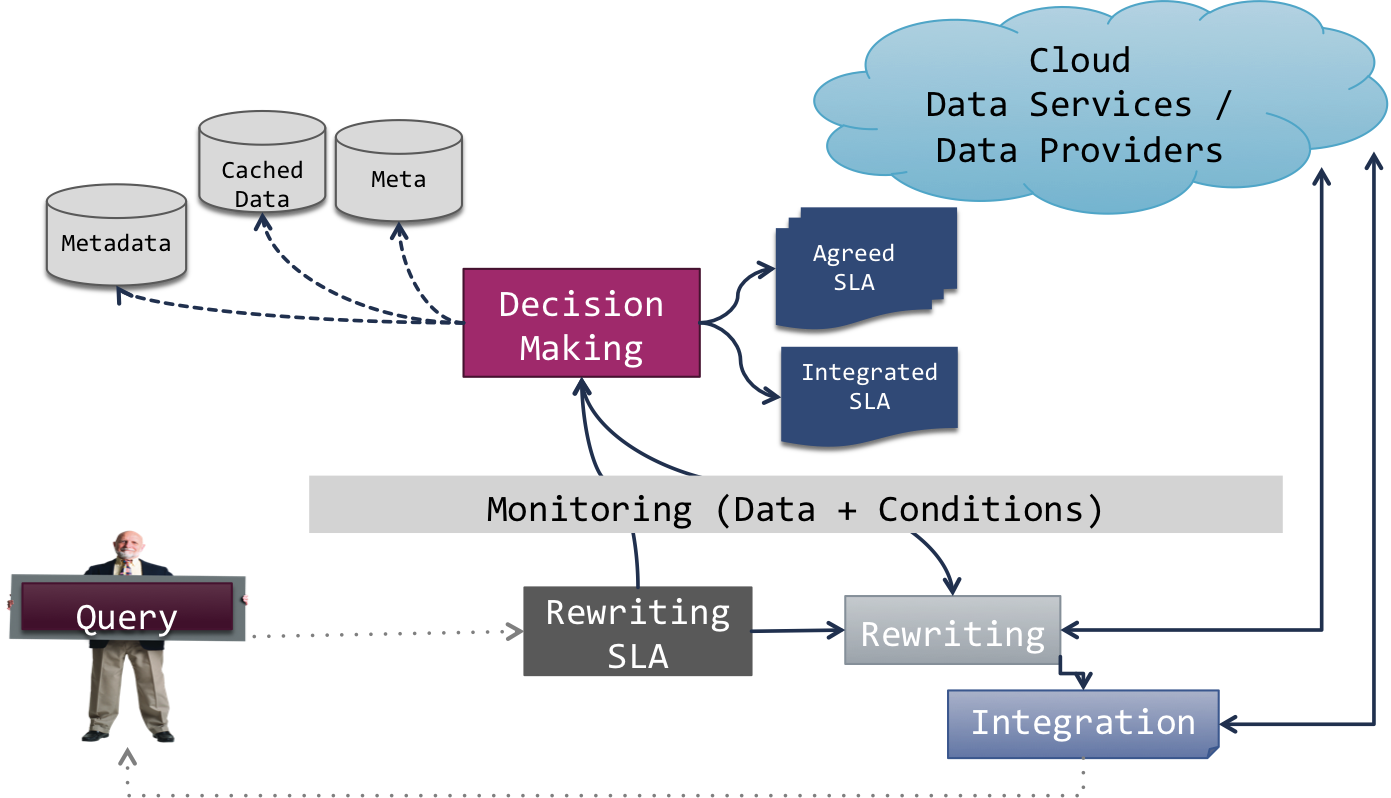
\includegraphics[width=3in]{figs/arch}
\caption{SLAG-DIAAS architecture}
\label{fig_sim}
\end{figure}

%(we can inspired from the Main concepts below to propose our SLA )
%
%
%In order to propose an SLA guided data provision and integration, we think about possible steps from the request to the delivery of the result sets. Indeed, let consider a request R launched by a user who specifies a number of constraints on the environment execution. Executing this query requires first a semantic analysis which will subdivide R into a set of sub-queries, in such a way that each sub-query can be processed by a DataService deployed on the cloud. The first stage of the process can be defined as a vertical mapping SLAs given the high level SLA described by the user (i.e. macroscopic constraints: execution time, pay / no pay, data reliability, data source). The system should be able to find relevant service compositions that respond to the query and, when combined, meet the constraints imposed by the user (High level SLA). 
%To meet this objective, it is necessary to compare the SLA services to combine, in order to check if their joint use is compatible with the individual SLA. This step may lead either to the rejection of integration in case of total incompatibility, or to a negotiation between SLA which will lead us to the proposal for a negotiated SLA integration and thus the need for an adaptive Template.
%The negotiation of this type of SLA depends strongly on the request sent and the services deployed at the arrival time of the application on the cloud. This negotiation can be expensive and may not scale well. It is therefore crucial to provide proactive mechanisms for optimizing the production of such SLA. We believe that the optimization of this process can occur at two levels, firstly at the level of SLA previously traded, and secondly at the level of partial or total results. Indeed, queries requesting the same services compositions will have clauses in their SLAs that are more conditions of use of the infrastructure (ie not touching the data). For two different queries, they will be negotiated in the same way. These previously negotiated SLAs are reusable. 
%In a second time, we think optimizing this process on the data storage mechanisms to cache intermediate results, individually or in partial or complete combination depending on the terms of SLA services (data access, intermediate storage capacity, cost of storage , etc ... ).
%To our knowledge, such an SLA composition and caching has not yet being used. Other works focus on the translation of SLA constraints from low to high level, or treat only of security SLA policies or semantic.

%\subsection{Subsection Heading Here}
%Subsection text here.

%Test of citation:~\cite{10.1109/CCGrid.2013.66}.
%
%\subsubsection{Subsubsection Heading Here}
%Subsubsection text here.
%
%\section{Type style and Fonts}
%Wherever Times is specified, Times Roman or Times New Roman may be used. If neither is available on your system, please use the font closest in appearance to Times. Avoid using bit-mapped fonts if possible. True-Type 1 or Open Type fonts are preferred. Please embed symbol fonts, as well, for math, etc.


% An example of a floating figure using the graphicx package.
% Note that \label must occur AFTER (or within) \caption.
% For figures, \caption should occur after the \includegraphics.
% Note that IEEEtran v1.7 and later has special internal code that
% is designed to preserve the operation of \label within \caption
% even when the captionsoff option is in effect. However, because
% of issues like this, it may be the safest practice to put all your
% \label just after \caption rather than within \caption{}.
%
% Reminder: the "draftcls" or "draftclsnofoot", not "draft", class
% option should be used if it is desired that the figures are to be
% displayed while in draft mode.
%
%\begin{figure}[!t]
%\centering
%\includegraphics[width=2.5in]{myfigure}
% where an .eps filename suffix will be assumed under latex, 
% and a .pdf suffix will be assumed for pdflatex; or what has been declared
% via \DeclareGraphicsExtensions.
%\caption{Simulation Results}
%\label{fig_sim}
%\end{figure}

% Note that IEEE typically puts floats only at the top, even when this
% results in a large percentage of a column being occupied by floats.


% An example of a double column floating figure using two subfigures.
% (The subfig.sty package must be loaded for this to work.)
% The subfigure \label commands are set within each subfloat command, the
% \label for the overall figure must come after \caption.
% \hfil must be used as a separator to get equal spacing.
% The subfigure.sty package works much the same way, except \subfigure is
% used instead of \subfloat.
%
%\begin{figure*}[!t]
%\centerline{\subfloat[Case I]\includegraphics[width=2.5in]{subfigcase1}%
%\label{fig_first_case}}
%\hfil
%\subfloat[Case II]{\includegraphics[width=2.5in]{subfigcase2}%
%\label{fig_second_case}}}
%\caption{Simulation results}
%\label{fig_sim}
%\end{figure*}
%
% Note that often IEEE papers with subfigures do not employ subfigure
% captions (using the optional argument to \subfloat), but instead will
% reference/describe all of them (a), (b), etc., within the main caption.


% An example of a floating table. Note that, for IEEE style tables, the 
% \caption command should come BEFORE the table. Table text will default to
% \footnotesize as IEEE normally uses this smaller font for tables.
% The \label must come after \caption as always.
%
%\begin{table}[!t]
%% increase table row spacing, adjust to taste
%\renewcommand{\arraystretch}{1.3}
% if using array.sty, it might be a good idea to tweak the value of
% \extrarowheight as needed to properly center the text within the cells
%\caption{An Example of a Table}
%\label{table_example}
%\centering
%% Some packages, such as MDW tools, offer better commands for making tables
%% than the plain LaTeX2e tabular which is used here.
%\begin{tabular}{|c||c|}
%\hline
%One & Two\\
%\hline
%Three & Four\\
%\hline
%\end{tabular}
%\end{table}


% Note that IEEE does not put floats in the very first column - or typically
% anywhere on the first page for that matter. Also, in-text middle ("here")
% positioning is not used. Most IEEE journals/conferences use top floats
% exclusively. Note that, LaTeX2e, unlike IEEE journals/conferences, places
% footnotes above bottom floats. This can be corrected via the \fnbelowfloat
% command of the stfloats package.


%\section{The integration SLA structure}
Figure~\ref{fig_integ} depicts how we extend the SLA structure in order to be able to capitalize on previous SLA negotiation. 
The yellow part of the schema gives an abstract presentation of SLA content necessary to describe our extension. 
Compared to standard SLA where two mandatory parties are concerned and a set of optional ones, we propose a set of parties formed by those (clouds, services, user) actors that are concerned in the data integration process. 
After the filtering process, the service selects the service composition that will cover the total result set. 
For each selected composition an integration SLA should be derived from the services and the user SLA. 
For each, obligations concerning the same items will be confronted to produce some new guaranties specified by the negotiation rules. 
The semantic analysis of the query allows to extract a set of concepts that are associated to the built \textit{Integration SLA}. 
These concepts are helpful in case of a future query that uses the same concepts and will allow to fetch for compositions that already meet the requirements of the user at first and the SLA of the entities implied thank to the Integration SLA.
\begin{figure}[!t]
\centering
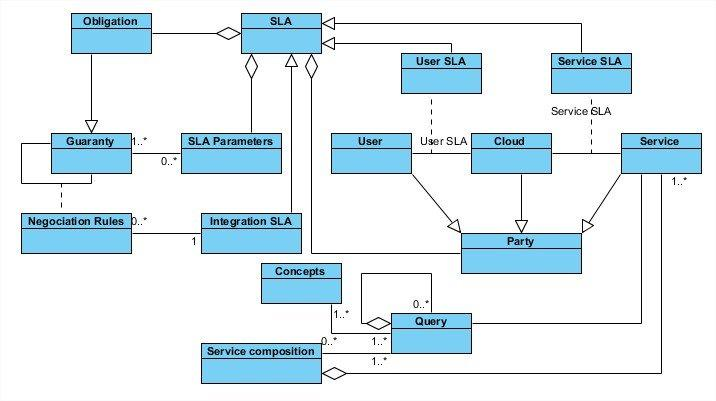
\includegraphics[width=3in]{figs/diagram}
\caption{SLA extension}
\label{fig_integ}
\end{figure}



\section{Conclusion}
This paper introduces the challenge of integrating data from distributed data services deployed on different cloud providers guided by service level agreement. 
The data integration problem is stated as a continuous data provision problem that has an associated economic cost and that uses automatic learning techniques for ensuring different qualities of delivered data (fresh, precise, partial).
Current big data settings impose today to consider SLA and different data delivery models. 
We believe that given the volume and the complexity of query evaluation that includes steps that imply greedy computations, it is important to combine and revisit well-known solutions and adapted to this contexts. 
We are currently developing the strategies and algorithms sketched here applied to energy consumption applications as the one described in the paper and also to elections and political campaign data integration in order to guide decision making on campaign strategies.

% conference papers do not normally have an appendix


% use section* for acknowledgement
%\section*{Acknowledgment}
%
%
%The authors would like to thank...
%more thanks here


% trigger a \newpage just before the given reference
% number - used to balance the columns on the last page
% adjust value as needed - may need to be readjusted if
% the document is modified later
%\IEEEtriggeratref{8}
% The "triggered" command can be changed if desired:
%\IEEEtriggercmd{\enlargethispage{-5in}}

% references section

% can use a bibliography generated by BibTeX as a .bbl file
% BibTeX documentation can be easily obtained at:
% http://www.ctan.org/tex-archive/biblio/bibtex/contrib/doc/
% The IEEEtran BibTeX style support page is at:
% http://www.michaelshell.org/tex/ieeetran/bibtex/
\bibliographystyle{IEEEtran}
% argument is your BibTeX string definitions and bibliography database(s)
\bibliography{example}
%
% <OR> manually copy in the resultant .bbl file
% set second argument of \begin to the number of references
% (used to reserve space for the reference number labels box)
%\begin{thebibliography}{1}
%
%\bibitem{IEEEhowto:kopka}
%H.~Kopka and P.~W. Daly, \emph{A Guide to \LaTeX}, 3rd~ed.\hskip 1em plus
%  0.5em minus 0.4em\relax Harlow, England: Addison-Wesley, 1999.
%
%\end{thebibliography}




% that's all folks
\end{document}


